

\tikzset{every picture/.style={line width=0.75pt}} %set default line width to 0.75pt

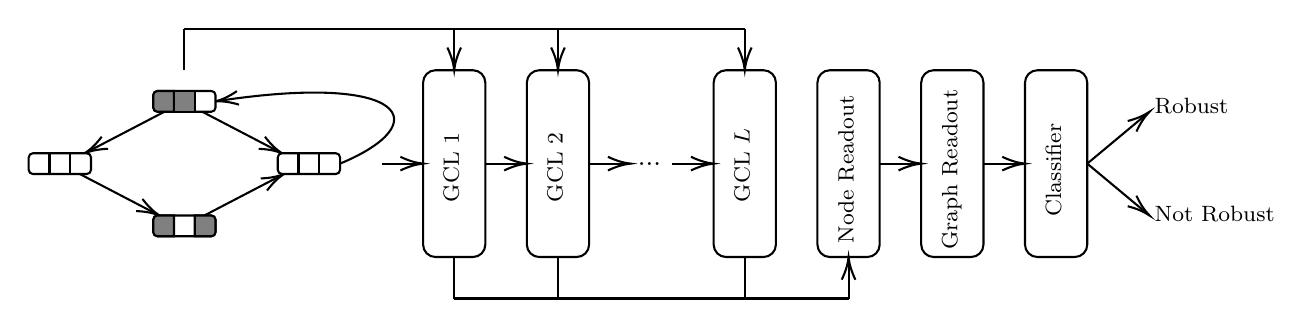
\begin{tikzpicture}[x=0.75pt,y=0.75pt,yscale=-1,xscale=1]
%uncomment if require: \path (0,222); %set diagram left start at 0, and has height of 222

%Straight Lines [id:da10249777348922673]
\draw    (105,55) -- (58.77,79.08) ;
\draw [shift={(57,80)}, rotate = 332.49] [color={rgb, 255:red, 0; green, 0; blue, 0 }  ][line width=0.75]    (10.93,-3.29) .. controls (6.95,-1.4) and (3.31,-0.3) .. (0,0) .. controls (3.31,0.3) and (6.95,1.4) .. (10.93,3.29)   ;
%Straight Lines [id:da8543699837088969]
\draw    (104,55) -- (150.23,79.08) ;
\draw [shift={(152,80)}, rotate = 207.51] [color={rgb, 255:red, 0; green, 0; blue, 0 }  ][line width=0.75]    (10.93,-3.29) .. controls (6.95,-1.4) and (3.31,-0.3) .. (0,0) .. controls (3.31,0.3) and (6.95,1.4) .. (10.93,3.29)   ;
%Curve Lines [id:da718018348959689]
\draw    (180,85) .. controls (226.69,65.62) and (212.66,40.97) .. (121.38,54.79) ;
\draw [shift={(120,55)}, rotate = 351.23] [color={rgb, 255:red, 0; green, 0; blue, 0 }  ][line width=0.75]    (10.93,-3.29) .. controls (6.95,-1.4) and (3.31,-0.3) .. (0,0) .. controls (3.31,0.3) and (6.95,1.4) .. (10.93,3.29)   ;
%Straight Lines [id:da40161395618619355]
\draw    (45,85) -- (91.23,109.08) ;
\draw [shift={(93,110)}, rotate = 207.51] [color={rgb, 255:red, 0; green, 0; blue, 0 }  ][line width=0.75]    (10.93,-3.29) .. controls (6.95,-1.4) and (3.31,-0.3) .. (0,0) .. controls (3.31,0.3) and (6.95,1.4) .. (10.93,3.29)   ;
%Straight Lines [id:da9404547371703709]
\draw    (105,115) -- (151.23,90.92) ;
\draw [shift={(153,90)}, rotate = 512.49] [color={rgb, 255:red, 0; green, 0; blue, 0 }  ][line width=0.75]    (10.93,-3.29) .. controls (6.95,-1.4) and (3.31,-0.3) .. (0,0) .. controls (3.31,0.3) and (6.95,1.4) .. (10.93,3.29)   ;
%Rounded Rect [id:dp8918717737625625]
\draw  [fill={rgb, 255:red, 255; green, 255; blue, 255 }  ,fill opacity=1 ] (30,82) .. controls (30,80.9) and (30.9,80) .. (32,80) -- (58,80) .. controls (59.1,80) and (60,80.9) .. (60,82) -- (60,88) .. controls (60,89.1) and (59.1,90) .. (58,90) -- (32,90) .. controls (30.9,90) and (30,89.1) .. (30,88) -- cycle ;
%Straight Lines [id:da2840220975641643]
\draw [fill={rgb, 255:red, 255; green, 255; blue, 255 }  ,fill opacity=1 ]   (40,80) -- (40,90) ;
%Straight Lines [id:da9928129104895596]
\draw [fill={rgb, 255:red, 255; green, 255; blue, 255 }  ,fill opacity=1 ]   (50,80) -- (50,90) ;

%Rounded Rect [id:dp657055048085913]
\draw  [fill={rgb, 255:red, 255; green, 255; blue, 255 }  ,fill opacity=1 ] (90,52) .. controls (90,50.9) and (90.9,50) .. (92,50) -- (118,50) .. controls (119.1,50) and (120,50.9) .. (120,52) -- (120,58) .. controls (120,59.1) and (119.1,60) .. (118,60) -- (92,60) .. controls (90.9,60) and (90,59.1) .. (90,58) -- cycle ;
%Straight Lines [id:da38800902985878216]
\draw [fill={rgb, 255:red, 255; green, 255; blue, 255 }  ,fill opacity=1 ]   (100,50) -- (100,60) ;
%Straight Lines [id:da35157806490529486]
\draw [fill={rgb, 255:red, 255; green, 255; blue, 255 }  ,fill opacity=1 ]   (110,50) -- (110,60) ;

%Rounded Rect [id:dp8042816045609678]
\draw  [fill={rgb, 255:red, 255; green, 255; blue, 255 }  ,fill opacity=1 ] (150,82) .. controls (150,80.9) and (150.9,80) .. (152,80) -- (178,80) .. controls (179.1,80) and (180,80.9) .. (180,82) -- (180,88) .. controls (180,89.1) and (179.1,90) .. (178,90) -- (152,90) .. controls (150.9,90) and (150,89.1) .. (150,88) -- cycle ;
%Straight Lines [id:da6303967094544072]
\draw [fill={rgb, 255:red, 255; green, 255; blue, 255 }  ,fill opacity=1 ]   (160,80) -- (160,90) ;
%Straight Lines [id:da38699794541515686]
\draw [fill={rgb, 255:red, 255; green, 255; blue, 255 }  ,fill opacity=1 ]   (170,80) -- (170,90) ;

%Rounded Rect [id:dp30617610846254983]
\draw  [fill={rgb, 255:red, 255; green, 255; blue, 255 }  ,fill opacity=1 ] (90,112) .. controls (90,110.9) and (90.9,110) .. (92,110) -- (118,110) .. controls (119.1,110) and (120,110.9) .. (120,112) -- (120,118) .. controls (120,119.1) and (119.1,120) .. (118,120) -- (92,120) .. controls (90.9,120) and (90,119.1) .. (90,118) -- cycle ;
%Straight Lines [id:da5849892704416262]
\draw [fill={rgb, 255:red, 255; green, 255; blue, 255 }  ,fill opacity=1 ]   (100,110) -- (100,120) ;
%Straight Lines [id:da5154765063607318]
\draw [fill={rgb, 255:red, 255; green, 255; blue, 255 }  ,fill opacity=1 ]   (110,110) -- (110,120) ;

%Rounded Same Side Corner Rect [id:dp16054859719249248]
\draw  [fill={rgb, 255:red, 128; green, 128; blue, 128 }  ,fill opacity=1 ] (92,120) .. controls (90.9,120) and (90,119.1) .. (90,118) -- (90,112) .. controls (90,110.9) and (90.9,110) .. (92,110) -- (100,110) .. controls (100,110) and (100,110) .. (100,110) -- (100,120) .. controls (100,120) and (100,120) .. (100,120) -- cycle ;
%Rounded Same Side Corner Rect [id:dp4777662533474829]
\draw  [fill={rgb, 255:red, 128; green, 128; blue, 128 }  ,fill opacity=1 ] (92,60) .. controls (90.9,60) and (90,59.1) .. (90,58) -- (90,52) .. controls (90,50.9) and (90.9,50) .. (92,50) -- (100,50) .. controls (100,50) and (100,50) .. (100,50) -- (100,60) .. controls (100,60) and (100,60) .. (100,60) -- cycle ;
%Rounded Rect [id:dp2612266462776953]
\draw   (220,46) .. controls (220,42.69) and (222.69,40) .. (226,40) -- (244,40) .. controls (247.31,40) and (250,42.69) .. (250,46) -- (250,124) .. controls (250,127.31) and (247.31,130) .. (244,130) -- (226,130) .. controls (222.69,130) and (220,127.31) .. (220,124) -- cycle ;
%Rounded Rect [id:dp6049233789003581]
\draw   (270,46) .. controls (270,42.69) and (272.69,40) .. (276,40) -- (294,40) .. controls (297.31,40) and (300,42.69) .. (300,46) -- (300,124) .. controls (300,127.31) and (297.31,130) .. (294,130) -- (276,130) .. controls (272.69,130) and (270,127.31) .. (270,124) -- cycle ;
%Rounded Rect [id:dp9219708545047745]
\draw   (360,46) .. controls (360,42.69) and (362.69,40) .. (366,40) -- (384,40) .. controls (387.31,40) and (390,42.69) .. (390,46) -- (390,124) .. controls (390,127.31) and (387.31,130) .. (384,130) -- (366,130) .. controls (362.69,130) and (360,127.31) .. (360,124) -- cycle ;
%Rounded Rect [id:dp06877784323777258]
\draw   (410,46) .. controls (410,42.69) and (412.69,40) .. (416,40) -- (434,40) .. controls (437.31,40) and (440,42.69) .. (440,46) -- (440,124) .. controls (440,127.31) and (437.31,130) .. (434,130) -- (416,130) .. controls (412.69,130) and (410,127.31) .. (410,124) -- cycle ;
%Straight Lines [id:da3242474162330802]
\draw    (105,20) -- (105,40) ;
%Straight Lines [id:da3678823594719134]
\draw    (105,20) -- (375,20) ;
%Straight Lines [id:da48488761692333315]
\draw    (200,85) -- (218,85) ;
\draw [shift={(220,85)}, rotate = 180] [color={rgb, 255:red, 0; green, 0; blue, 0 }  ][line width=0.75]    (10.93,-3.29) .. controls (6.95,-1.4) and (3.31,-0.3) .. (0,0) .. controls (3.31,0.3) and (6.95,1.4) .. (10.93,3.29)   ;
%Straight Lines [id:da7353824116605796]
\draw    (250,85) -- (268,85) ;
\draw [shift={(270,85)}, rotate = 180] [color={rgb, 255:red, 0; green, 0; blue, 0 }  ][line width=0.75]    (10.93,-3.29) .. controls (6.95,-1.4) and (3.31,-0.3) .. (0,0) .. controls (3.31,0.3) and (6.95,1.4) .. (10.93,3.29)   ;
%Straight Lines [id:da621667250955845]
\draw    (300,85) -- (318,85) ;
\draw [shift={(320,85)}, rotate = 180] [color={rgb, 255:red, 0; green, 0; blue, 0 }  ][line width=0.75]    (10.93,-3.29) .. controls (6.95,-1.4) and (3.31,-0.3) .. (0,0) .. controls (3.31,0.3) and (6.95,1.4) .. (10.93,3.29)   ;
%Straight Lines [id:da0389620564663371]
\draw    (340,85) -- (358,85) ;
\draw [shift={(360,85)}, rotate = 180] [color={rgb, 255:red, 0; green, 0; blue, 0 }  ][line width=0.75]    (10.93,-3.29) .. controls (6.95,-1.4) and (3.31,-0.3) .. (0,0) .. controls (3.31,0.3) and (6.95,1.4) .. (10.93,3.29)   ;
%Straight Lines [id:da49854406681907104]
\draw    (235,20) -- (235,38) ;
\draw [shift={(235,40)}, rotate = 270] [color={rgb, 255:red, 0; green, 0; blue, 0 }  ][line width=0.75]    (10.93,-3.29) .. controls (6.95,-1.4) and (3.31,-0.3) .. (0,0) .. controls (3.31,0.3) and (6.95,1.4) .. (10.93,3.29)   ;
%Straight Lines [id:da3320143976606864]
\draw    (285,20) -- (285,38) ;
\draw [shift={(285,40)}, rotate = 270] [color={rgb, 255:red, 0; green, 0; blue, 0 }  ][line width=0.75]    (10.93,-3.29) .. controls (6.95,-1.4) and (3.31,-0.3) .. (0,0) .. controls (3.31,0.3) and (6.95,1.4) .. (10.93,3.29)   ;
%Straight Lines [id:da0031583922795141994]
\draw    (375,20) -- (375,38) ;
\draw [shift={(375,40)}, rotate = 270] [color={rgb, 255:red, 0; green, 0; blue, 0 }  ][line width=0.75]    (10.93,-3.29) .. controls (6.95,-1.4) and (3.31,-0.3) .. (0,0) .. controls (3.31,0.3) and (6.95,1.4) .. (10.93,3.29)   ;
%Straight Lines [id:da6752204950269405]
\draw    (440,85) -- (458,85) ;
\draw [shift={(460,85)}, rotate = 180] [color={rgb, 255:red, 0; green, 0; blue, 0 }  ][line width=0.75]    (10.93,-3.29) .. controls (6.95,-1.4) and (3.31,-0.3) .. (0,0) .. controls (3.31,0.3) and (6.95,1.4) .. (10.93,3.29)   ;
%Rounded Rect [id:dp17194220548550754]
\draw   (460,46) .. controls (460,42.69) and (462.69,40) .. (466,40) -- (484,40) .. controls (487.31,40) and (490,42.69) .. (490,46) -- (490,124) .. controls (490,127.31) and (487.31,130) .. (484,130) -- (466,130) .. controls (462.69,130) and (460,127.31) .. (460,124) -- cycle ;
%Straight Lines [id:da6487892442997589]
\draw    (490,85) -- (508,85) ;
\draw [shift={(510,85)}, rotate = 180] [color={rgb, 255:red, 0; green, 0; blue, 0 }  ][line width=0.75]    (10.93,-3.29) .. controls (6.95,-1.4) and (3.31,-0.3) .. (0,0) .. controls (3.31,0.3) and (6.95,1.4) .. (10.93,3.29)   ;
%Straight Lines [id:da05300848730559804]
\draw    (235,130) -- (235,150) ;
%Straight Lines [id:da3909014389203407]
\draw    (285,130) -- (285,150) ;
%Straight Lines [id:da6126666581003337]
\draw    (375,130) -- (375,150) ;
%Straight Lines [id:da02140734221954288]
\draw    (425,150) -- (425,132) ;
\draw [shift={(425,130)}, rotate = 450] [color={rgb, 255:red, 0; green, 0; blue, 0 }  ][line width=0.75]    (10.93,-3.29) .. controls (6.95,-1.4) and (3.31,-0.3) .. (0,0) .. controls (3.31,0.3) and (6.95,1.4) .. (10.93,3.29)   ;
%Straight Lines [id:da951914950788185]
\draw    (235,150) -- (425,150) ;
%Rounded Rect [id:dp02585435349200571]
\draw   (510,46) .. controls (510,42.69) and (512.69,40) .. (516,40) -- (534,40) .. controls (537.31,40) and (540,42.69) .. (540,46) -- (540,124) .. controls (540,127.31) and (537.31,130) .. (534,130) -- (516,130) .. controls (512.69,130) and (510,127.31) .. (510,124) -- cycle ;
%Straight Lines [id:da6345268220344737]
\draw    (540,85) -- (568.46,108.72) ;
\draw [shift={(570,110)}, rotate = 219.81] [color={rgb, 255:red, 0; green, 0; blue, 0 }  ][line width=0.75]    (10.93,-3.29) .. controls (6.95,-1.4) and (3.31,-0.3) .. (0,0) .. controls (3.31,0.3) and (6.95,1.4) .. (10.93,3.29)   ;
%Straight Lines [id:da603900144364321]
\draw    (540,85) -- (568.46,61.28) ;
\draw [shift={(570,60)}, rotate = 500.19] [color={rgb, 255:red, 0; green, 0; blue, 0 }  ][line width=0.75]    (10.93,-3.29) .. controls (6.95,-1.4) and (3.31,-0.3) .. (0,0) .. controls (3.31,0.3) and (6.95,1.4) .. (10.93,3.29)   ;
%Shape: Rectangle [id:dp46978661229215835]
\draw  [fill={rgb, 255:red, 128; green, 128; blue, 128 }  ,fill opacity=1 ] (100,50) -- (110,50) -- (110,60) -- (100,60) -- cycle ;
%Rounded Same Side Corner Rect [id:dp24282480800994288]
\draw  [fill={rgb, 255:red, 128; green, 128; blue, 128 }  ,fill opacity=1 ] (118,110) .. controls (119.1,110) and (120,110.9) .. (120,112) -- (120,118) .. controls (120,119.1) and (119.1,120) .. (118,120) -- (110,120) .. controls (110,120) and (110,120) .. (110,120) -- (110,110) .. controls (110,110) and (110,110) .. (110,110) -- cycle ;

% Text Node
\draw (228.5,105) node [anchor=north west][inner sep=0.75pt]  [font=\footnotesize,rotate=-270] [align=left] {GCL 1};
% Text Node
\draw (278.5,105) node [anchor=north west][inner sep=0.75pt]  [font=\footnotesize,rotate=-270] [align=left] {GCL 2};
% Text Node
\draw (322,83) node [anchor=north west][inner sep=0.75pt]  [align=left] {...};
% Text Node
\draw (368.5,105) node [anchor=north west][inner sep=0.75pt]  [font=\footnotesize,rotate=-270] [align=left] {GCL $\displaystyle L$};
% Text Node
\draw (418.5,125) node [anchor=north west][inner sep=0.75pt]  [font=\footnotesize,rotate=-270] [align=left] {Node Readout};
% Text Node
\draw (468.5,128) node [anchor=north west][inner sep=0.75pt]  [font=\footnotesize,rotate=-270] [align=left] {Graph Readout};
% Text Node
\draw (518.5,112) node [anchor=north west][inner sep=0.75pt]  [font=\footnotesize,rotate=-270] [align=left] {Classifier};
% Text Node
\draw (571,52) node [anchor=north west][inner sep=0.75pt]  [font=\footnotesize] [align=left] {Robust};
% Text Node
\draw (571,104) node [anchor=north west][inner sep=0.75pt]  [font=\footnotesize] [align=left] {Not Robust};


\end{tikzpicture}